\chapter{Introduzione}
Nell'ambito della sicurezza informatica, la gestione delle vulnerabilità nei software è diventata un pilastro fondamentale per garantire l'integrità e la protezione dei sistemi informativi. Con l'avvento delle tecnologie cloud e la diffusione di metodologie di sviluppo agile, gli strumenti di scansione delle vulnerabilità sono diventati strumenti indispensabili per gli sviluppatori e i professionisti della sicurezza. Questo report si propone di esplorare e confrontare due dei più rilevanti strumenti nel panorama della sicurezza informatica: Trivy e Snyk. Entrambi gli strumenti hanno guadagnato notorietà per la loro capacità di fornire analisi dettagliate e soluzioni alle vulnerabilità di sicurezza in applicazioni e container, ma presentano approcci, caratteristiche e punti di forza distinti.

\section*{Trivy}

Trivy\footnote{\url{https://github.com/aquasecurity/trivy}}, sviluppato da Aqua Security, è uno scanner di vulnerabilità open source semplice ma completo, che si distingue per la sua facilità d'uso e la capacità di integrarsi in vari ambienti di sviluppo e pipeline CI/CD. Le sue funzionalità includono la scansione di repository Git, filesystem e configurazioni Infrastructure as Code (IaC), che rendono quindi Trivy uno strumento versatile sia per sviluppatori che per i team di sicurezza. Trivy è inoltre altamente personalizzabile, con la possibilità, ad esempio, di includere proprie vulnerabilità appena scoperte nell'analisi dei container.

\section*{Snyk}

Snyk\footnote{\url{https://snyk.io}} si posiziona come una soluzione SaaS "chiavi in mano" per tutto ciò che concerne le vulnerabilità nello sviluppo software. Diviso in quattro componenti principali, rende possibile l'analisi delle vulnerabilità sin dai primi momenti di scrittura del codice. Inoltre, punta a semplificare la gestione delle vulnerabilità nelle dipendenze, attuando ove possibile risoluzioni automatiche. Utilizzabile sia da interfaccia Web che da linea di comando, Snyk mira a dotare anche ai team più piccoli degli strumenti e dei consigli per affrontare le vulnerabilità all'interno del loro codice, delle dipendenze open source, dei container e delle configurazioni IaC.

\section{Processi di scansione}
\subsection{Trivy}
I tool effettuano il processo di scansione delle vulnerabilità in container Docker in modi diversi:

\textbf{Trivy} utilizza il comando di scansione \texttt{trivy image} per eseguire la scansione di un'immagine Docker\cite{trivy_docs}. Questo comando esegue automaticamente tre funzioni:
\begin{itemize}
   \item \textbf{Download del database delle vulnerabilità}: Trivy scarica automaticamente l'ultima versione del database delle vulnerabilità dalla repository ufficiale.
   \item \textbf{Scansione dell'immagine}: Trivy esegue la scansione dell'immagine Docker specificata, identificando e classificando le vulnerabilità presenti nei pacchetti e nelle librerie. Nel processo di scansione, Trivy analizza i file presenti nell'immagine, identificando le versioni dei pacchetti e confrontandole con il database di vulnerabilità. Nel processo, vengono scansionate quattro categorie di problemi di sicurezza:
         \begin{itemize}
            \item \textbf{Vulnerabilità}: problemi di sicurezza noti e documentati, che possono essere sfruttati da attaccanti per compromettere l'integrità e la disponibilità del sistema.
            \item \textbf{Configurazioni errate}: errori di configurazione e di implementazione che possono esporre il sistema a rischi di sicurezza.
            \item \textbf{Segreti e chiavi di accesso}: presenza di segreti e chiavi di accesso non crittografate all'interno dell'immagine, che possono essere sfruttati da attaccanti per ottenere accesso non autorizzato al sistema.
            \item \textbf{Licenze:} presenza di licenze non conformi o non autorizzate all'interno dell'immagine, che possono esporre il sistema a rischi legali e di sicurezza.
         \end{itemize}
         Di default, Trivy esegue la scansione di tutte e quattro le categorie, ma è possibile specificare una categoria specifica da scansionare utilizzando l'opzione \texttt{--scanners <vuln\_type>}.

   \item \textbf{Generazione del report}: Trivy genera un report dettagliato delle vulnerabilità rilevate, classificandole in base al loro grado di gravità e fornendo informazioni dettagliate sulle azioni consigliate per mitigarle. La gravità di una vulnerabilità è assegnata tramite due fattori principali:
         \begin{itemize}
            \item Principalmente, si fa affidamento al livello di gravità riportato dal vendor per tale vulnerabilità.
            \item In caso il vendor non riporti la categoria della vulnerabilità, Trivy fa affidamento alla gravità assegnata dal database NVD.
            \item In caso anche il database NVD non riporti la categoria della vulnerabilità, Trivy la riporta come di categoria UNKNOWN.
         \end{itemize}
\end{itemize}
\subsection{Snyk}
Snyk opera invece tramite un approccio differente\cite{snyk_docs}. Invece di utilizzare un unico comando per performare tutte le azioni di scansione, Snyk è suddiviso in quattro componenti principali, ognuna dedicata ad un momento differente nello sviluppo software:
\begin{itemize}
   \item \textbf{Snyk Code:} componente relativo all'analisi statica. Connettendo il proprio sistema di gestione del codice sorgente (es. Git) a Snyk Code tramite l'apposita integrazione, il proprio progetto viene analizzato automaticamente, per identificare i possibili problemi di sicurezza presenti nel codice. Gli eventuali problemi di sicurezza rilevati vengono notificati all'utente tramite l'interfaccia web di Snyk, con un'evidenziazione delle linee di codice interessate e delle azioni consigliate per mitigare i problemi, come riportato in Figura \ref{fig:snyk_code}.
         \begin{figure}[H]
            \centering
            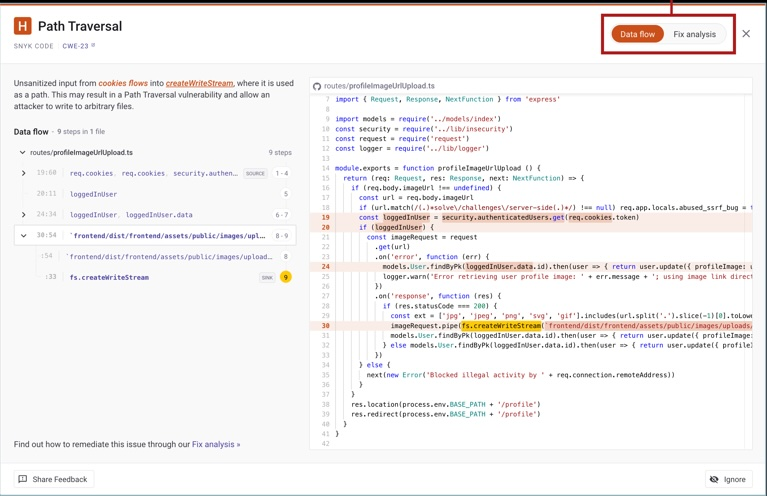
\includegraphics[width=0.8\textwidth]{immagini/capitolo1/snyk_code.jpg}
            \caption{Risultato della scansione del codice sorgente con Snyk Code}
            \label{fig:snyk_code}
         \end{figure}
   \item \textbf{Snyk Container:} il vero e proprio strumento per l'analisi delle vulnerabilità nei container. Questo processo, avviabile tramite il comando \texttt{snyk test}, è suddiviso in tre fasi principali:
         \begin{itemize}
            \item \textbf{Download dell'immagine}: l'immagine viene automaticamente scaricata in locale per permetterne l'analisi.
            \item \textbf{Ottenimento della lista del software installato:} Snyk cerca il software installato all'interno dell'immagine. La ricerca viene effettuata in base a tre criteri:
                  \begin{itemize}
                     \item Software installato tramite package manager (es. apt, yum, apk)
                     \item Software comunemente installato, e residente in posizioni predefinite
                     \item Applicazioni basate sulla presenza di un file manifest (es. package.json, requirements.txt)
                  \end{itemize}
            \item \textbf{Invio delle vulnerabilità a Snyk:} La lista del software trovato viene inviata tramite API a Snyk, la quale confronta i dati con il suo database di vulnerabilità. Un report contenente le vulnerabilità trovate viene quindi restituito all'utente.
         \end{itemize}
         Snyk assegna inoltre ad ogni vulnerabilità un cosiddetto \textbf{priority score}, ovvero un punteggio da 0 a 1000 che indica la priorità con la quale la vulnerabilità dovrebbe essere risolta. Questo punteggio è calcolato in base a diversi fattori, tra cui la gravità della vulnerabilità, la popolarità del pacchetto e la presenza di exploit pubblici.
         In Figura \ref{fig:snyk_container} è riportata una vulnerabilità rilevata tramite analisi con Snyk Container. È possibile notare, sulla destra, anche il Priority Score.
         \begin{figure}[H]
            \centering
            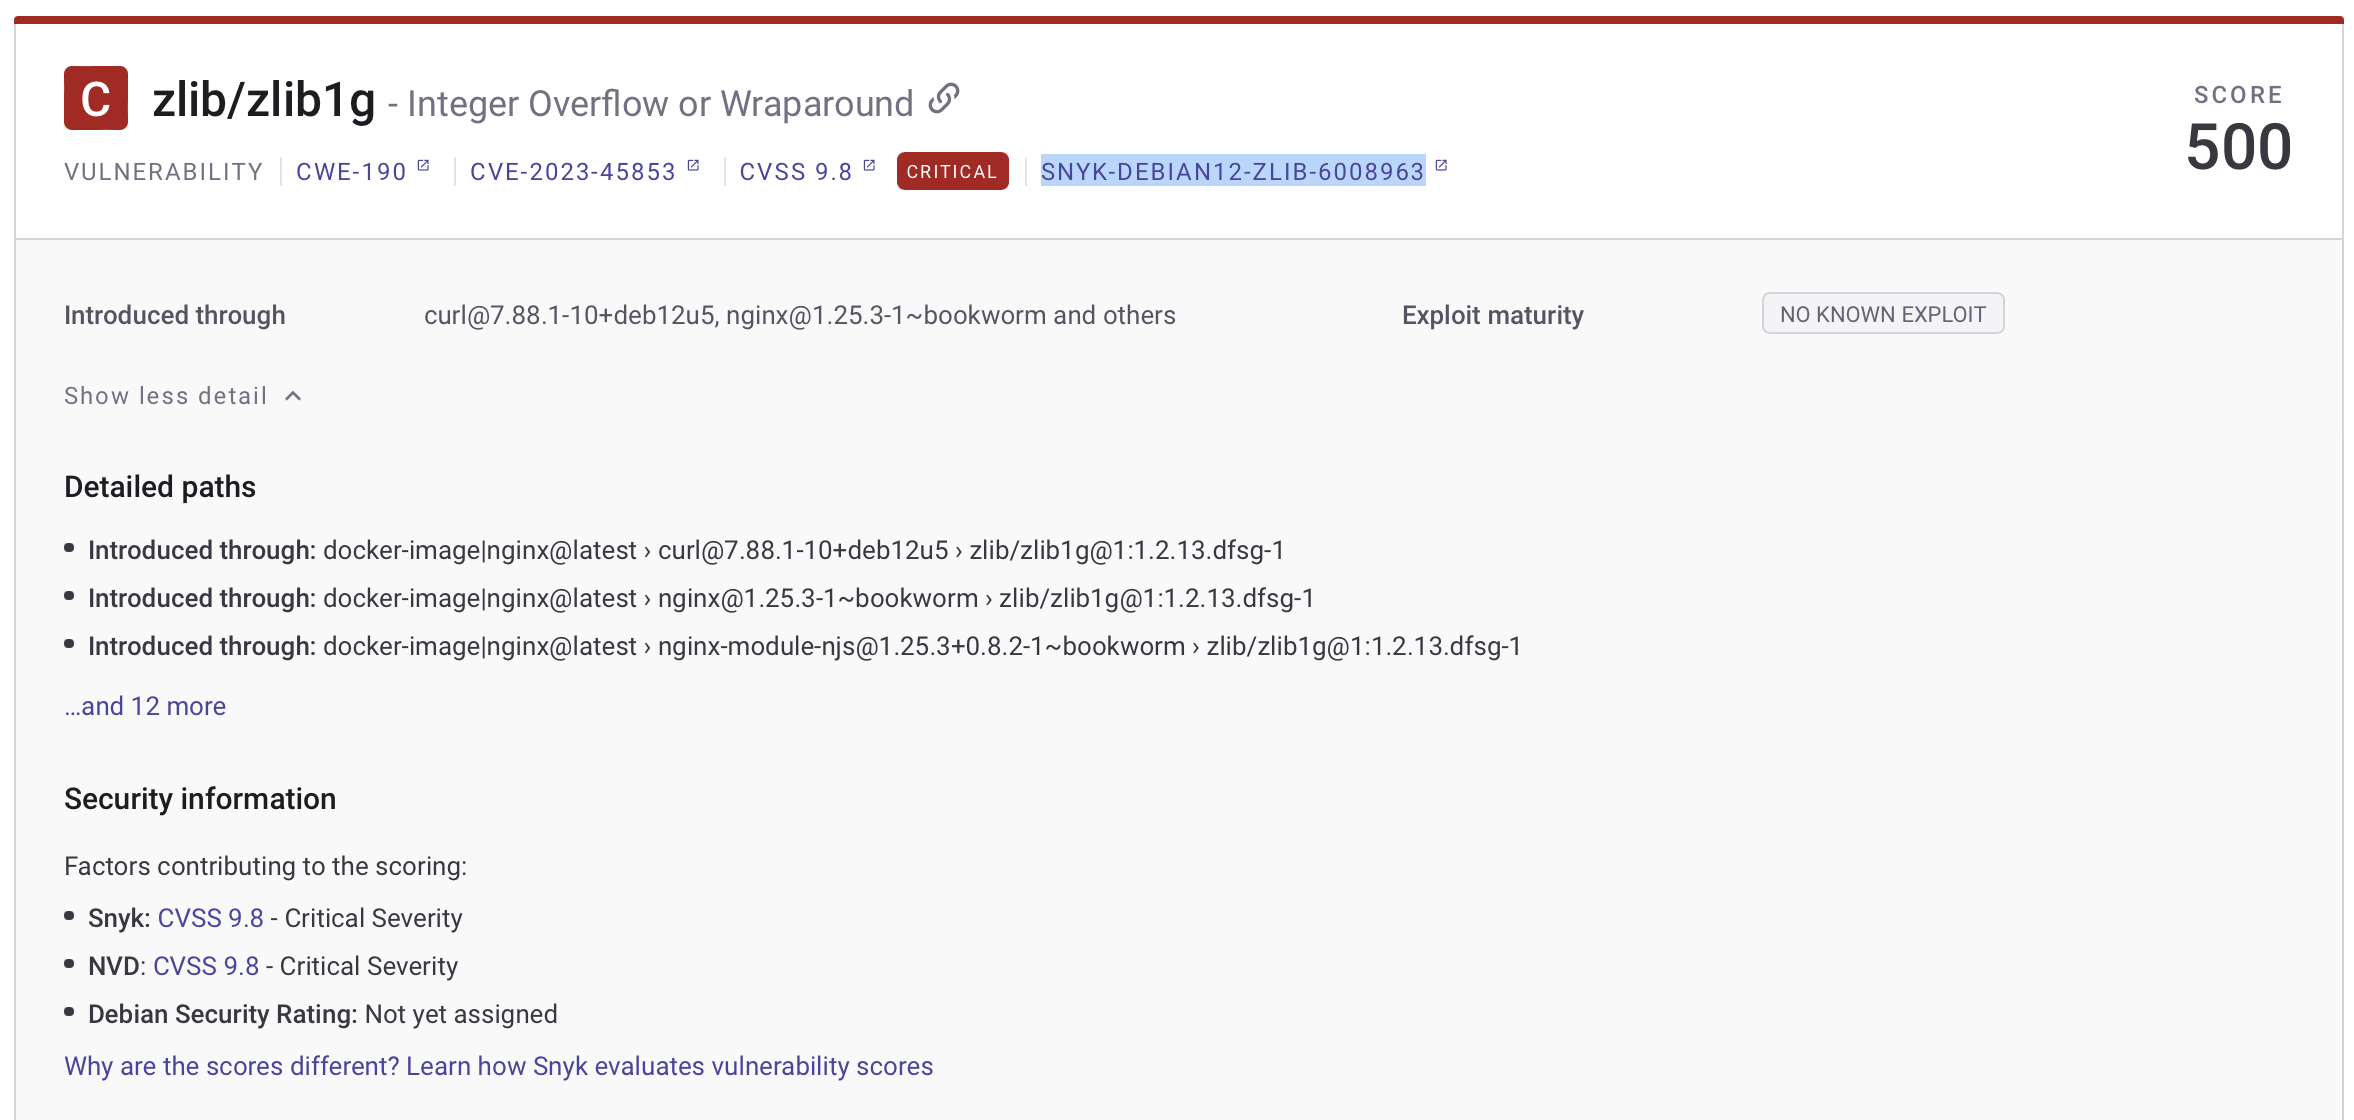
\includegraphics[width=0.8\textwidth]{immagini/capitolo1/snyk_container.png}
            \caption{Vulnerabilità rilevata tramite l'analisi con Snyk Container}
            \label{fig:snyk_container}
         \end{figure}
   \item \textbf{Snyk Open Source:} Uno strumento di analisi delle vulnerabilità per le dipendenze open source presenti nel progetto, che identifica e classifica le vulnerabilità presenti nelle librerie e nei pacchetti utilizzati all'interno del codice sorgente. Snyk Open Source è in grado di eseguire la scansione delle dipendenze open source, identificando le vulnerabilità e fornendo informazioni dettagliate sulle azioni consigliate per mitigarle.
   \item \textbf{Snyk Infrastructure as Code:} Snyk IaC è uno strumento di analisi delle vulnerabilità per le configurazioni Infrastructure as Code (IaC), che identifica e classifica possibili problemi presenti nei file di configurazione di Terraform, CloudFormation e altri strumenti di automazione dell'infrastruttura. È inoltre possibile impostare Snyk per confrontare lo stato specificato su Terraform con lo stato effettivamente in uso su un cloud provider, per individuare qualsiasi possibile variazione non desiderata.

\end{itemize}